% Generated by empirical_bloomberg_20261030/make_empirical_section.py. Supplementary notes
% distributed with the replication package (paper/supplement_20261030.tex), not submitted.
\section{Observation conventions and source audit}
\label{supp:conventions}
No observations are forward filled. Bloomberg-reported dates and repeated values
are retained, and a constant reported value is not proof of an independently refreshed
quote. Levels are joined before differencing. Increments may span one to four
calendar days (exactly one day for the crypto series). ACF lags count observations,
not a common calendar duration. Daily closes may differ in time across sources, so
regressions measure end-of-day association. Price references use capital and split
adjustment with cash-dividend adjustment disabled, and a separately fetched
cash-adjusted series supplies a sensitivity check. Ten-year yields, quoted in
percent, are multiplied by 100 before differencing. The yield is a proxy for
MOVE's option basket. USO's changing portfolio and index-methodology changes limit
invariant interpretations.

The Bloomberg histories agree with the previously used Cboe/Yahoo/archive sources
on most dates and differ on a few. Table~\ref{tab:provider-overlap} compares levels
on identical dates. The largest OVX difference is 23.75 points on 25 November 2011
(Cboe 69.12, Bloomberg 45.37) and the largest MOVE difference is 29.06 points on
15 March 2023 (archive 169.65, Bloomberg 198.71). Their causes have not been
established. The Bloomberg observations are primary throughout.

\begin{table}[htbp]\centering\small\begin{tabular}{@{}l r r r r r@{}}\toprule Series & Overlap $N$ & Median $|\Delta|$ & Max $|\Delta|$ & Old score & BBG score\\\midrule

VIX & 6731 & 0.00000 & 0.010 & 0.1580 & 0.1580 \\

OVX & 4255 & 0.00000 & 23.750 & 0.0566 & 0.0565 \\

MOVE & 5121 & 0.00000 & 29.060 & -0.1217 & -0.1210 \\

\bottomrule\end{tabular}
\caption{Source differences in index points (MOVE: yield-volatility bp). The last two
columns are GIG minus Heston-marginal held-out mean log scores on identical dates
with a 70/30 chronological split, isolating the source effect from the longer sample.}
\label{tab:provider-overlap}\end{table}

Excluding both increments touching a disputed date (absolute source difference above 0.005 points for VIX or 0.1 for OVX and MOVE) changes the span-65 positive-beta frequencies as follows: VIX: 0.0 to 0.0\%; OVX: 17.0 to 17.0\%; MOVE: 63.9 to 64.1\%. These thresholds were set after inspecting the discrepancies, so this is a diagnostic rather than a cleaned sample.

Enabling cash-dividend adjustment changes a native span-65 positive frequency by at most 0.51 percentage points across the Cboe panel. A short sensitivity beginning 10 February 2025, with local fits restarted at that boundary, is retained in the package, and it is not evidence that methodology changes caused a regime shift. Regime summaries, 130- and 500-block interval sensitivities and all training and evaluation dates are stored with the results.

\subsection{DVOL observations and UTC alignment}
\label{supp:dvol}
The primary crypto series are BTC and ETH DVOL daily OHLC closes, targeting
30-day annualised volatility. They are not the legacy ATM files reported below.
Each contains 2,045 positive finite daily closes from 24 March 2021 to 28 October
2026, with no missing or duplicated dates. Index points are divided by 100 for
estimation and multiplied by 100 for percentage-volatility figures and tables.
The timestamp of a daily DVOL candle labels its start. Aggregating the 24 hourly
candles of 28 October reproduces that day's daily OHLC for each asset, and aggregating
the preceding day does not. Accordingly, the candle labelled $d$ is paired with
the underlying USD spot index at $(d+1)$ 00:00 UTC. Differences of adjacent pairs
therefore measure the same daily interval. There are 2,044 paired increments,
1,980 span-65 estimates and 1,785 span-260 estimates per asset, and no levels are filled.

The USD index observations are the \texttt{index\_price} field in Deribit's
hourly perpetual funding-history response, not perpetual prices or funding
returns.\footnote{\url{https://docs.deribit.com/api-reference/market-data/public-get_funding_rate_history}.
Raw responses are cached in requests of at most 28 days. Every required midnight
is present, and consecutive hourly records reproduce the prior \texttt{index\_price}
in \texttt{prev\_index\_price} exactly. DVOL endpoints and methodology are cited in
the main paper.} The chart-history endpoint was rejected because its overlapping
values changed with chart resolution. Reference provenance and UTC timestamps are
recorded alongside the aligned daily inputs. The older 08:00 UTC ATM references
are not used for DVOL regressions.

The estimators are the same as in the main comparison: trailing regressions with
an intercept, level-pair ACFs, and training-only maximum likelihood followed by
one chronological 70/30 split. Both histories train on 1,431 observations through
21 February 2025 and evaluate on 614 observations from 22 February 2025.
Table~\ref{tab:dvol-acf} reports persistence on the daily crypto calendar. The
survival plots in Figure~\ref{fig:dvol-density-acf} show the shift to lower
volatility: neither evaluation sample exceeds its training 95th percentile.
A zero count is not a confidence bound for unseen extreme events. The BTC
GIG-minus-Heston and GIG-minus-3/2 intervals include zero, whereas ETH favours GIG over
Heston and the 3/2 and lognormal families over GIG. The same signs of
these interval conclusions hold with 130-observation score blocks. These are
marginal transfer diagnostics, not pricing-model or stress-risk rankings.

\begin{table}[htbp]\centering\small\begin{tabular}{@{}l r r r r@{}}\toprule Series & Lag (days) & Correlation & 250-block interval & 500-block interval\\\midrule

BTC DVOL & 1 & 0.985 & [0.967, 0.990] & [0.967, 0.990] \\

BTC DVOL & 5 & 0.942 & [0.882, 0.967] & [0.863, 0.967] \\

BTC DVOL & 20 & 0.844 & [0.676, 0.897] & [0.634, 0.902] \\

BTC DVOL & 60 & 0.764 & [0.389, 0.848] & [0.362, 0.845] \\

BTC DVOL & 120 & 0.703 & [0.343, 0.809] & [0.178, 0.845] \\

ETH DVOL & 1 & 0.986 & [0.970, 0.991] & [0.970, 0.991] \\

ETH DVOL & 5 & 0.944 & [0.887, 0.963] & [0.854, 0.959] \\

ETH DVOL & 20 & 0.834 & [0.715, 0.875] & [0.683, 0.867] \\

ETH DVOL & 60 & 0.716 & [0.495, 0.791] & [0.457, 0.769] \\

ETH DVOL & 120 & 0.600 & [0.339, 0.756] & [0.328, 0.732] \\

\bottomrule\end{tabular}\caption{DVOL level correlations and pointwise 95\% lag-pair block intervals. All dates are retained, so observation lags equal calendar-day lags. Source: Deribit, March 2021--October 2026.}\label{tab:dvol-acf}\end{table}

\begin{figure}[p]\centering
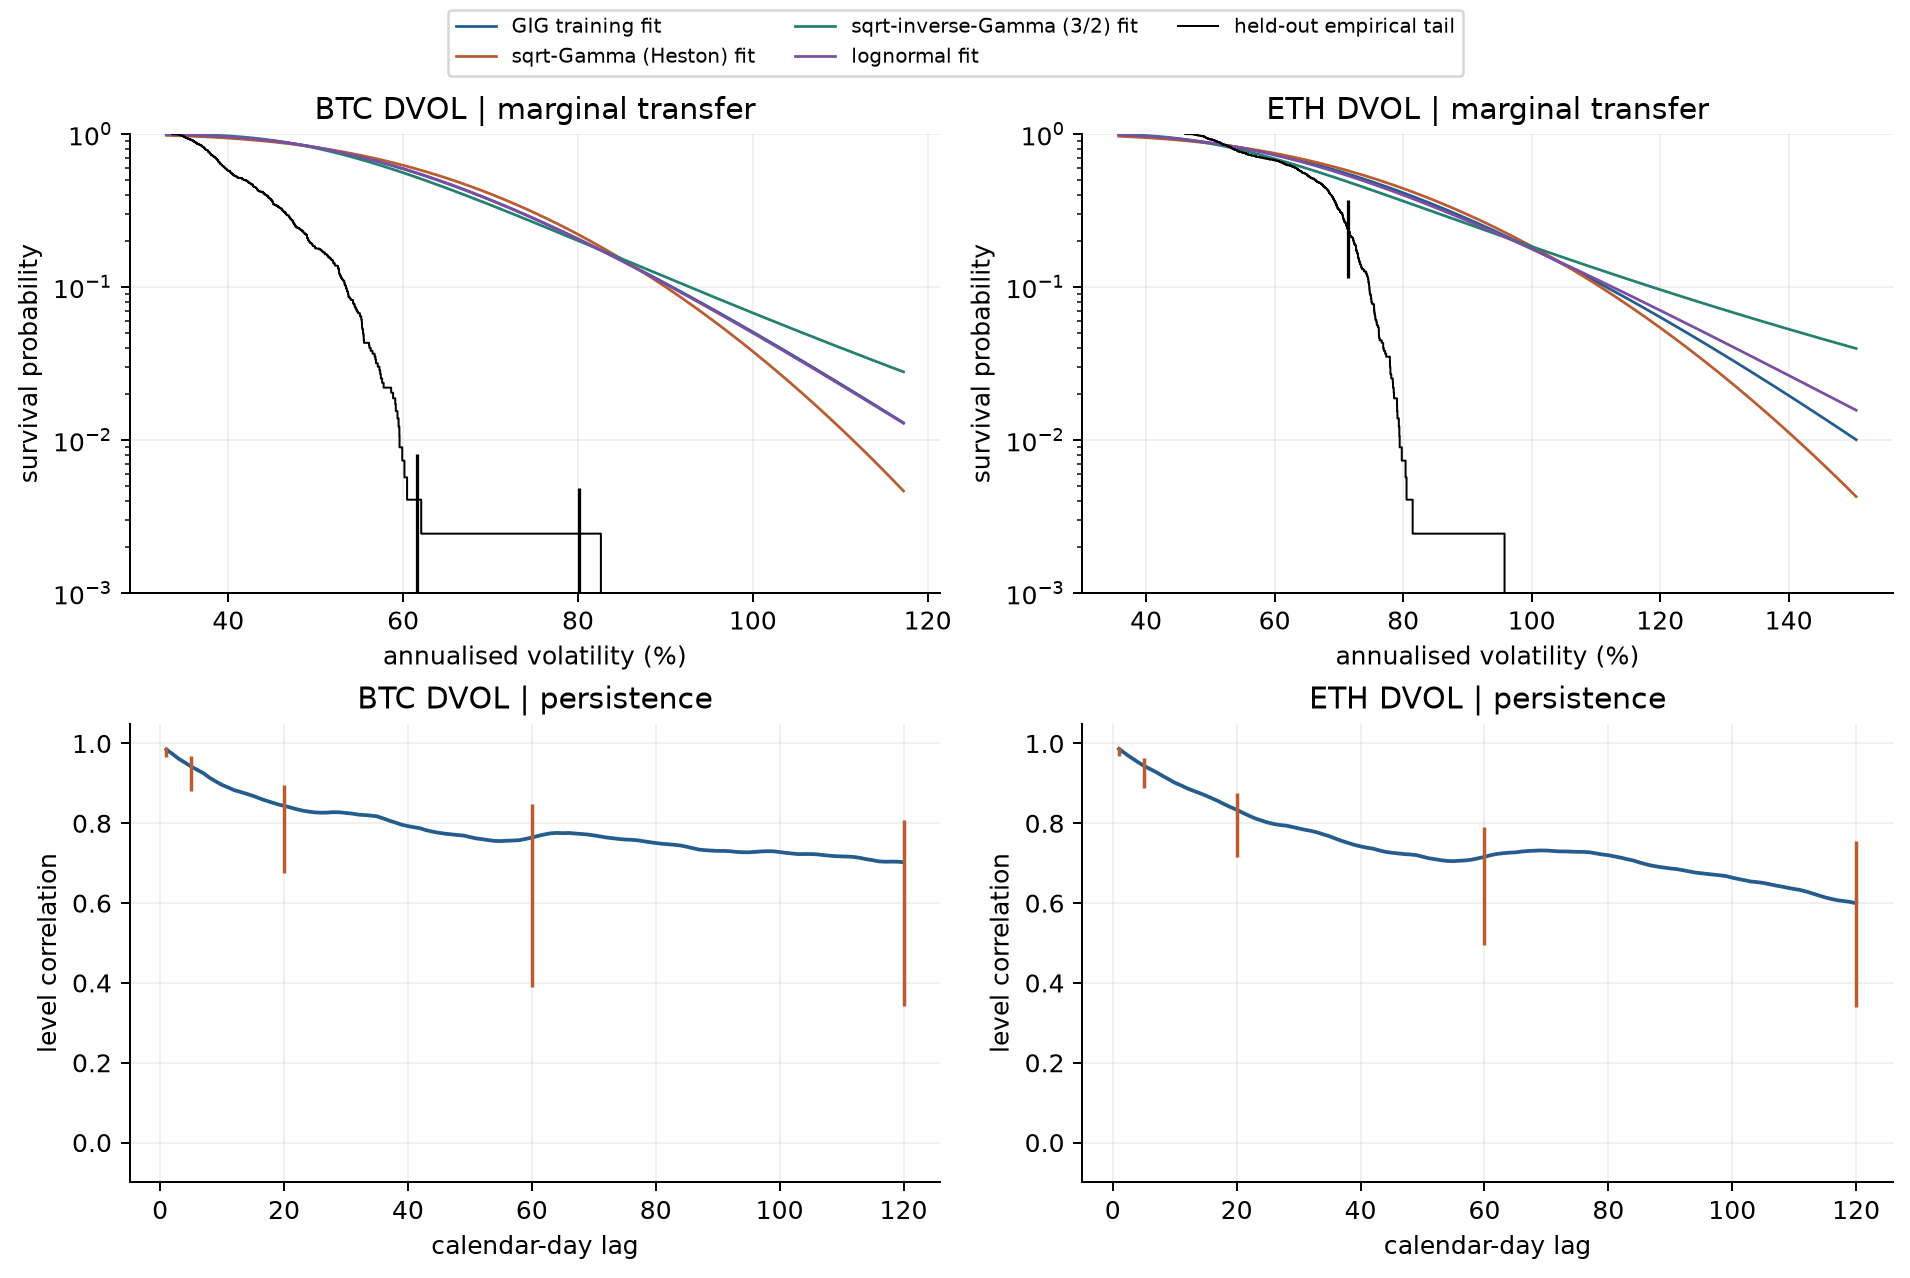
\includegraphics[width=\textwidth,height=.65\textheight,keepaspectratio]{figures/dvol_diagnostics_20261030/dvol_density_acf.png}
\caption{BTC and ETH DVOL: training-fitted survival functions and held-out tails (top), and level correlations with pointwise 95\% lag-pair block intervals (bottom). The survival axis is truncated below 0.001. Bars in the upper panels use training quantiles and 65-day blocks; lower panels use 250-day blocks. Source: Deribit.}\label{fig:dvol-density-acf}\end{figure}

\section{Newer, relaunched and unavailable Cboe candidates}
\label{supp:newer}
Newly launched or relaunched histories are not pooled into the established panel,
because some historical levels are back-calculated. Table~\ref{tab:cboe-new} reports
their coverage. VXLQD returned no Bloomberg history and VXIEF returned a stale
history ending in 2020. Neither is treated as a current observation. VVIX is
volatility of volatility and is excluded from the price-volatility panel. BITVX
measures Bitcoin ETF option-implied volatility and does not replace the legacy
crypto ATM series.

\begin{table}[htbp]\centering\small\begin{tabular}{@{}l l r r r@{}}\toprule Index & Current launch/relaunch & Available $N$ & Post-launch $N$ & Post-launch mean\\\midrule

VXSLV & 2025-06-16 & 3929 & 345 & 49.39 \\

VXHYG & 2025-06-16 & 2859 & 345 & 6.95 \\

VXFXI & 2025-11-03 & 1181 & 248 & 25.08 \\

VXGDX & 2025-11-03 & 1181 & 248 & 47.63 \\

VXUNG & 2025-06-16 & 1209 & 345 & 56.71 \\

VXLQD & 2025-08-25 & 0 & --- & --- \\

VXIEF & 2025-08-25 & 1312 & --- & --- \\

VXSMH & 2025-11-03 & 1210 & 248 & 44.49 \\

BITVX & 2026-03-23 & 456 & 153 & 45.67 \\

\bottomrule\end{tabular}\caption{Newer and relaunched Cboe cohort. Means are annualised percentage price volatility. Available counts can include backfilled history. Missing cells are deliberately not estimated.}\label{tab:cboe-new}\end{table}

\section{Legacy BTC and ETH ATM implied-volatility series}
\label{supp:crypto}
The retained BTC and ETH ATM implied-volatility files, observed daily at 08:00 UTC
from Deribit, lack expiry, tenor and day-count metadata. The earlier seven-day
designation cannot be verified and the series are not the DVOL index. Two invalid
ETH observations are removed. We report the same diagnostics as for the primary
cohort, with crypto increments restricted to exactly one calendar day, and treat
them as exploratory.

\begin{table}[htbp]\centering\small\setlength{\tabcolsep}{4pt}
\begin{tabular}{@{}l P{39mm} r P{31mm} r@{}}\toprule Series & Sample & $N$ & Native mean (interval) & Common mean\\\midrule

BTC & 2019-03-30 to 2024-05-05 & 1864 & 65.2 [56.0, 73.6] & 65.6 \\

ETH & 2019-03-30 to 2024-03-01 & 1797 & 76.7 [62.7, 89.5] & 77.2 \\

\bottomrule\end{tabular}\caption{Coverage of the legacy crypto ATM series. Means are percentage volatility; native-mean intervals use 250-observation blocks. The archived common means use 1230 common dates from 2019-04-01 to 2024-03-01 across the Bloomberg and legacy ATM series, independently of the new five-index DVOL comparison.}\label{tab:crypto-data}\end{table}

\begin{table}[htbp]\centering\small\begin{tabular}{@{}l r r r r@{}}\toprule Series & Span & Estimates & Positive (\%, interval) & Lower band $>0$ (\%)\\\midrule

BTC & 65 & 1799 & 42.2 [28.0, 56.7] & 16.8 \\

BTC & 260 & 1604 & 33.5 [8.7, 61.5] & 5.9 \\

ETH & 65 & 1730 & 36.1 [22.1, 49.1] & 11.1 \\

ETH & 260 & 1535 & 22.0 [4.0, 40.6] & 3.4 \\

\bottomrule\end{tabular}\caption{Positive observed-beta frequencies for the legacy crypto series, with conventions as in the main text.}\label{tab:crypto-beta}\end{table}

\begin{table}[htbp]\centering\small\setlength{\tabcolsep}{3pt}\begin{tabular}{@{}l P{24mm} P{36mm} P{36mm} P{36mm}@{}}\toprule Series & GIG law & GIG minus Heston & GIG minus 3/2 & GIG minus lognormal\\\midrule

BTC & Interior GIG & -0.300 [-0.818, 0.055] & 0.315 [0.014, 0.671] & -0.133 [-0.303, -0.004] \\

ETH & Inverse-Gamma & -1.351 [-2.849, -0.222] & 1.094 [0.215, 2.406] & -0.682 [-1.439, -0.138] \\

\bottomrule\end{tabular}\caption{Held-out mean log-score differences for the legacy crypto series. ETH's lower-volatility evaluation period exposes poor transfer of every training density, and BTC has no evaluation observation above its training 95th percentile.}\label{tab:crypto-scores}\end{table}

Lag-120 level correlations are BTC: 0.173, ETH: 0.326.

\begin{figure}[p]\centering
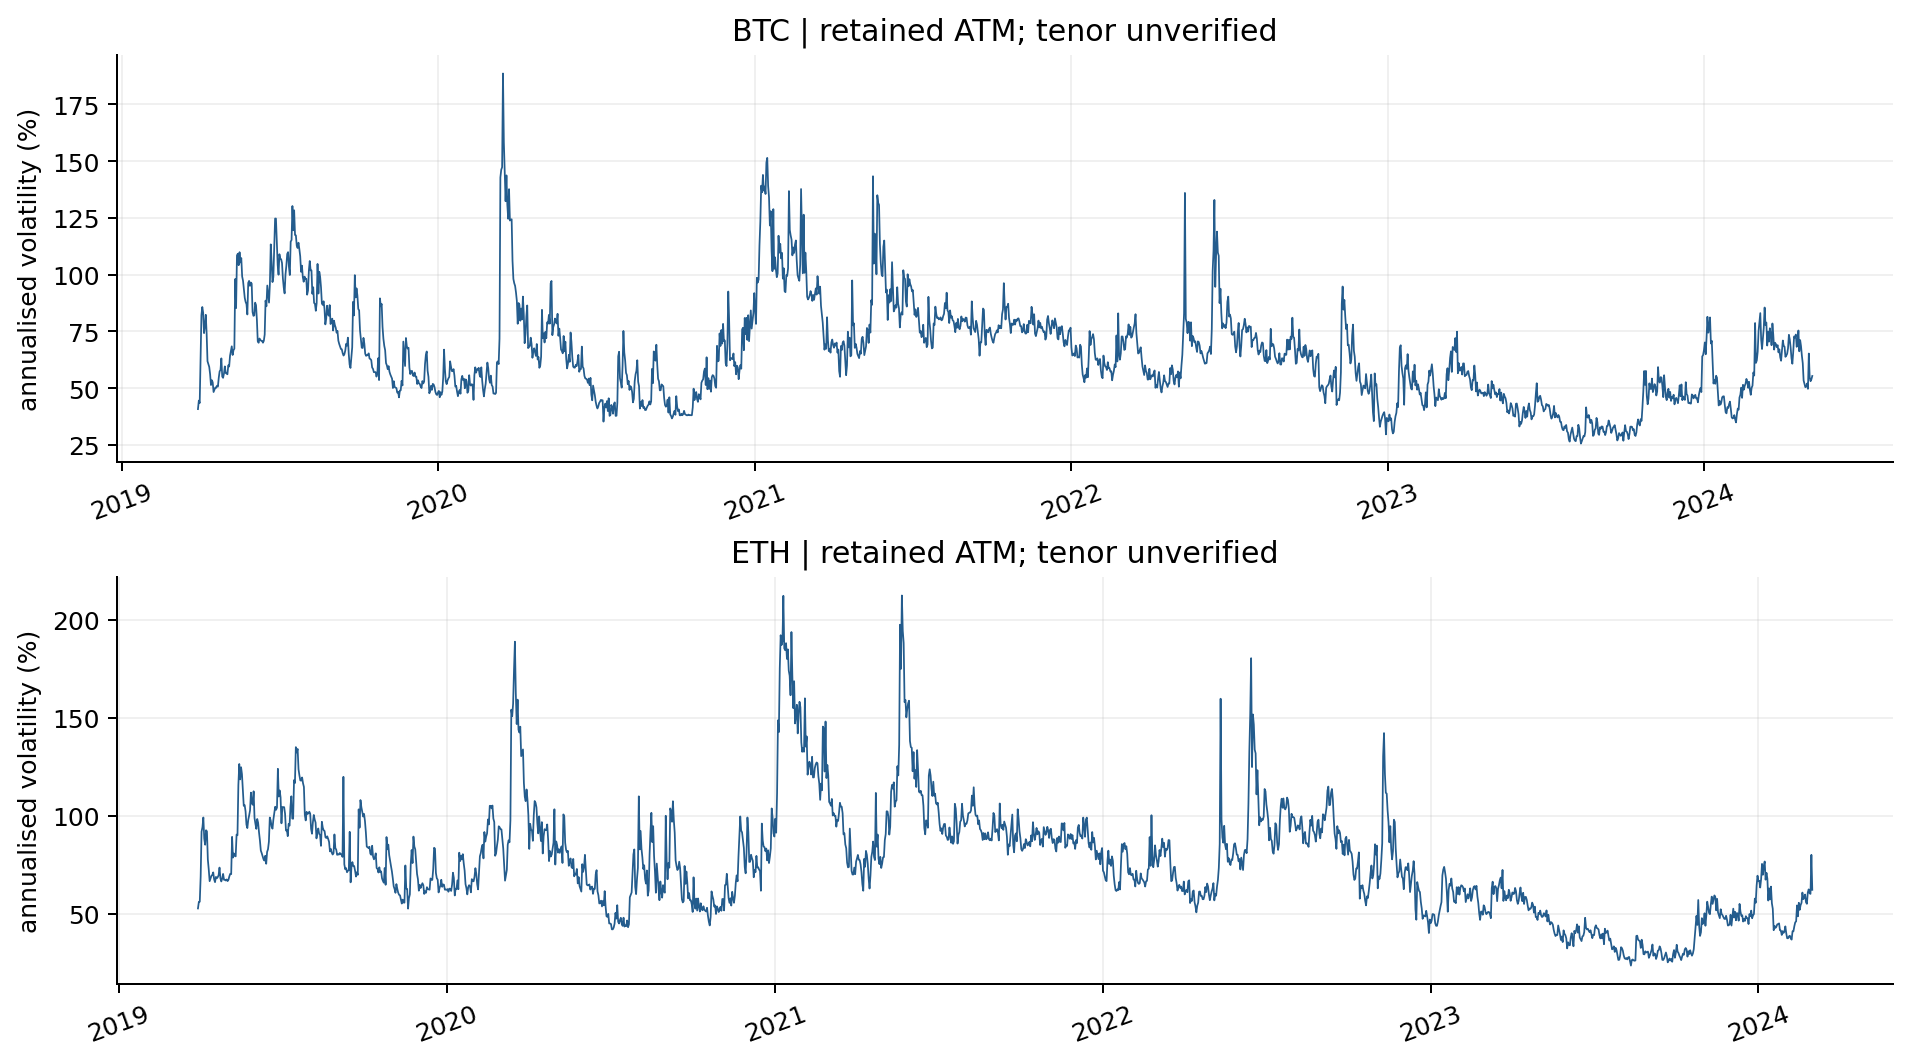
\includegraphics[width=\textwidth,height=.45\textheight,keepaspectratio]{figures/empirical_bloomberg_20261030/levels_crypto.png}
\caption{Legacy BTC and ETH ATM implied-volatility histories.}\label{fig:crypto-levels}\end{figure}

\begin{figure}[p]\centering
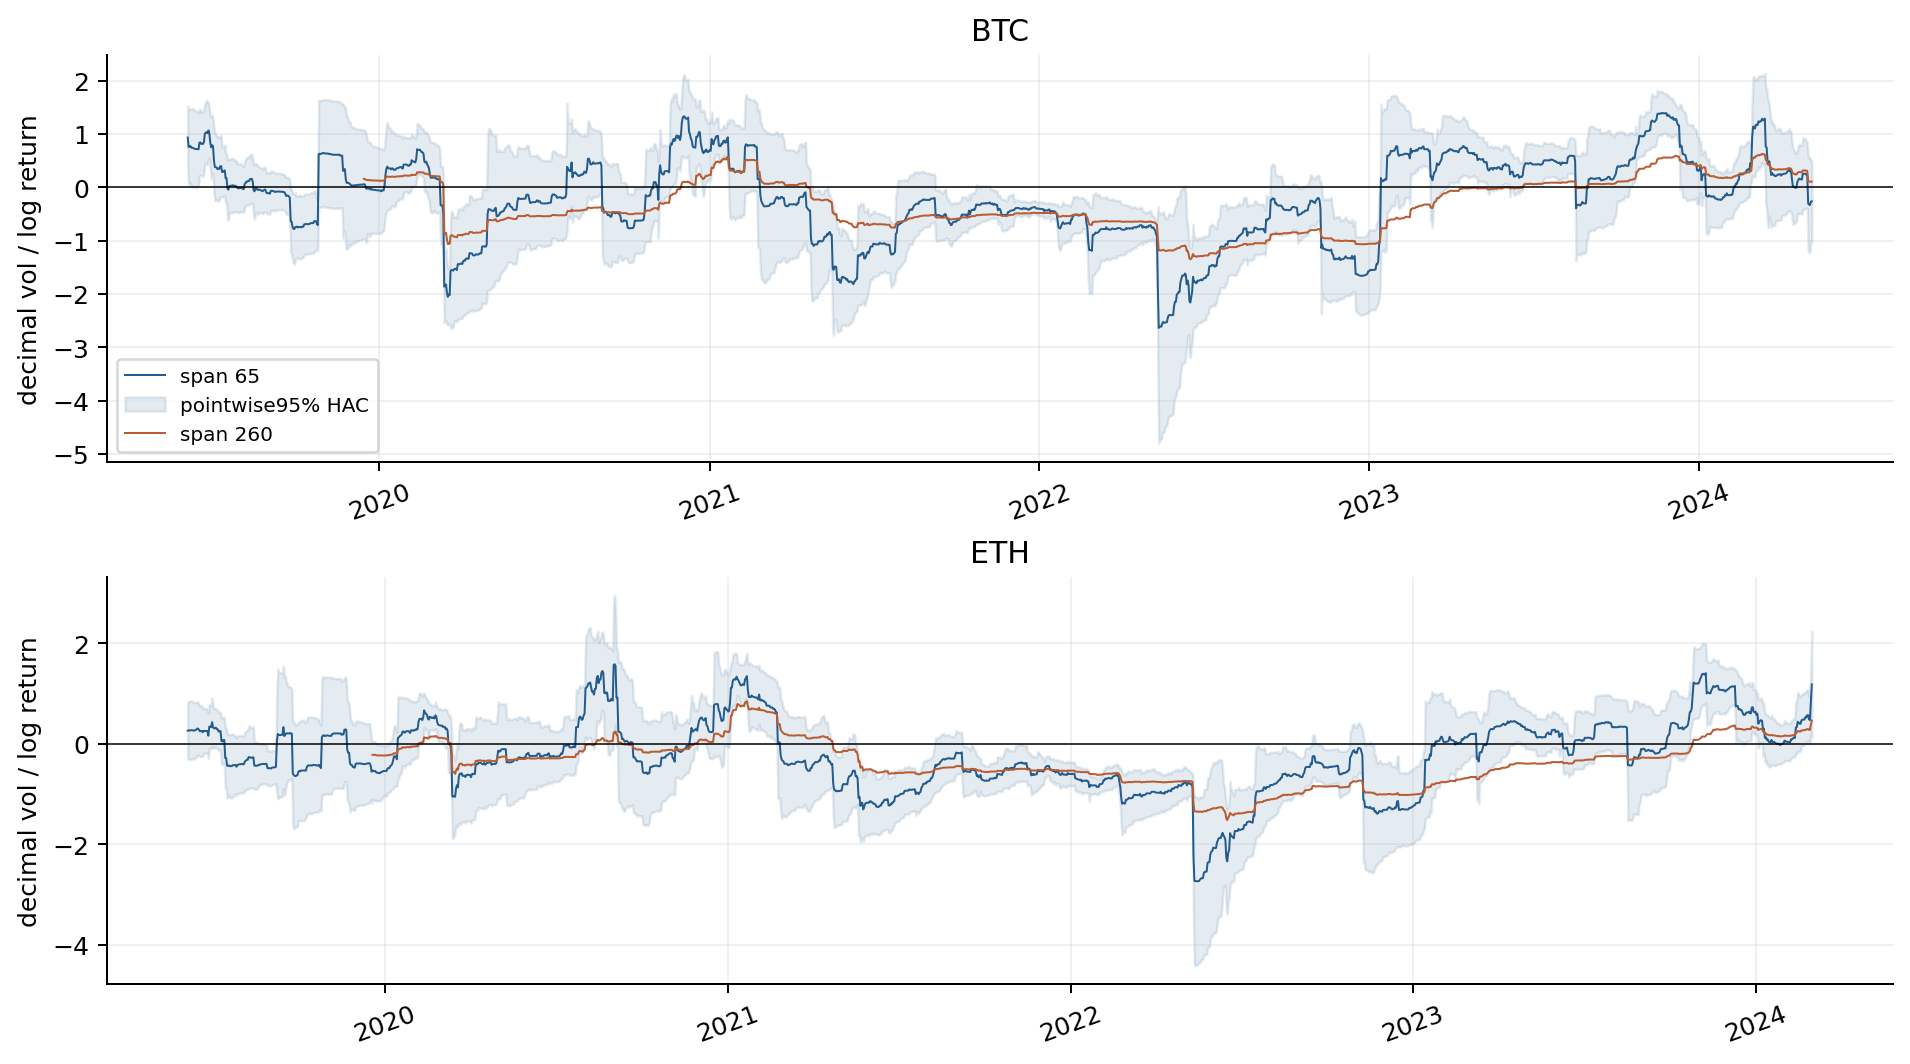
\includegraphics[width=\textwidth,height=.45\textheight,keepaspectratio]{figures/empirical_bloomberg_20261030/beta_crypto.png}
\caption{Observed level-beta paths for BTC and ETH. Blue: span 65 with pointwise 95\% HAC bands; orange: span 260.}\label{fig:crypto-beta}\end{figure}

\begin{figure}[p]\centering
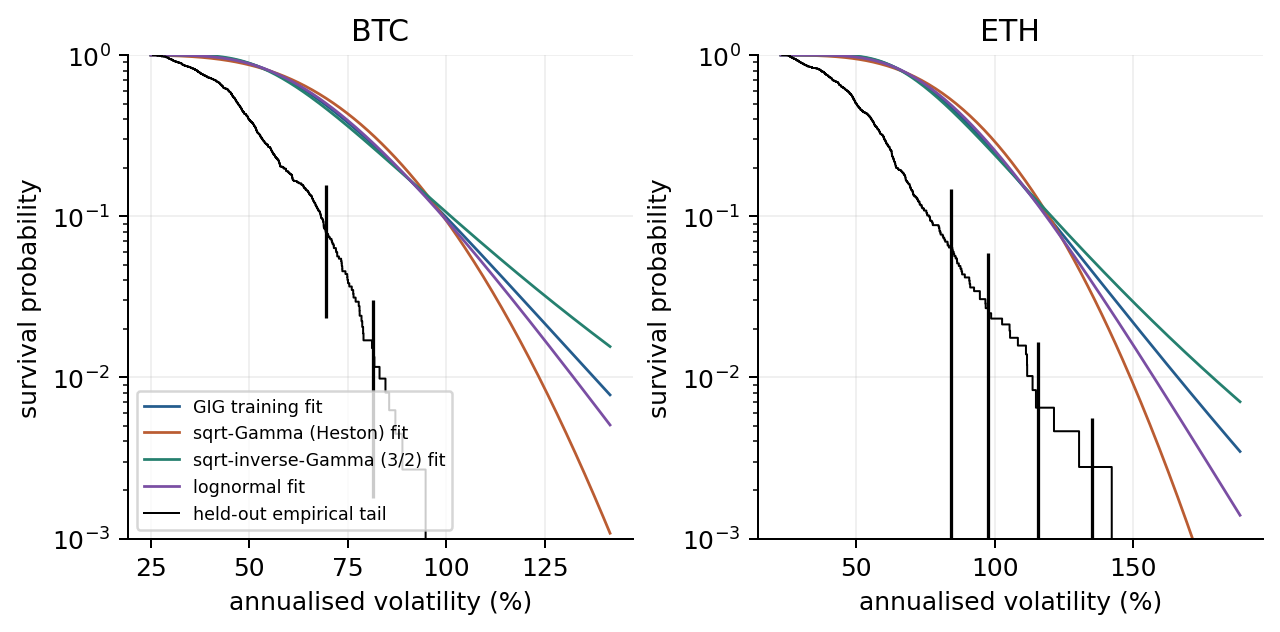
\includegraphics[width=\textwidth,height=.45\textheight,keepaspectratio]{figures/empirical_bloomberg_20261030/density_crypto.png}
\caption{Training-fitted survival functions and held-out tails for BTC and ETH.}\label{fig:crypto-density}\end{figure}

\begin{figure}[p]\centering
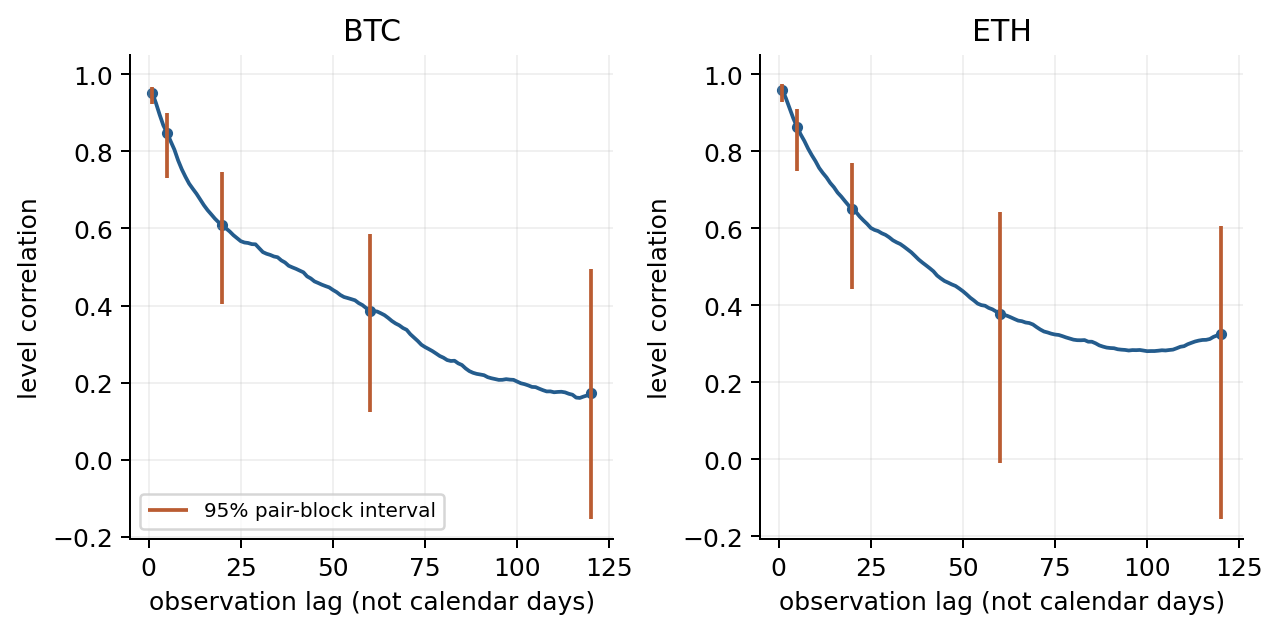
\includegraphics[width=\textwidth,height=.45\textheight,keepaspectratio]{figures/empirical_bloomberg_20261030/acf_crypto.png}
\caption{Lag correlations of BTC and ETH ATM volatility with pointwise 95\% lag-pair block intervals.}\label{fig:crypto-acf}\end{figure}
